% LTeX: enabled=false
% Komparator: V_in am +, V_ref am - (passt zu signalverlauf_komparator.png: V_out,max wenn V_in > V_ref)
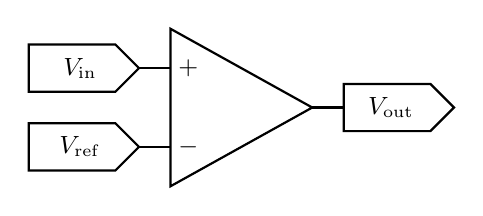
\begin{tikzpicture}[x=0.5cm,y=0.5cm,font=\small,thick]
  % OpAmp
  \draw (0,-2) -- (0,2) -- (3.6,0) -- cycle;
  \node at (0.45,1) {$+$};
  \node at (0.45,-1) {$-$};
  % Eingänge
  \draw (-3.6,1.6) -- (-1.4,1.6) -- (-0.8,1) -- (-1.4,0.4) -- (-3.6,0.4) -- cycle;
  \node at (-2.3,1) {$V_{\rm in}$};
  \draw (-0.8,1) -- (0,1);
  \draw (-3.6,-0.4) -- (-1.4,-0.4) -- (-0.8,-1) -- (-1.4,-1.6) -- (-3.6,-1.6) -- cycle;
  \node at (-2.3,-1) {$V_{\rm ref}$};
  \draw (-0.8,-1) -- (0,-1);
  % Ausgang
  \draw (3.6,0) -- (4.4,0);
  \draw (4.4,0.6) -- (6.6,0.6) -- (7.2,0) -- (6.6,-0.6) -- (4.4,-0.6) -- cycle;
  \node at (5.6,0) {$V_{\rm out}$};
\end{tikzpicture}
